

\section{Programs}
Every example program in this section uses R7 as a stack pointer which is initialised to the by the program to 0x07D0 using the LUI and LLI instructions.
It is possible a stack is not required in which case no initialisation is needed and R7 can be used as a general purpose register. \todo{surely this should be in the register description section}





\subsection{Multiply}
\label{sec:multiply}
The code for the multiply program is held in Appendix~\ref{sec:multiply_appendix} listing~\ref{lst:multiply.asm}.
A sixteen bit number is read from input switches and then split in to lower and upper bytes which are then multiplied.
The resulting sixteen bit word is written to the LEDs before reaching a terminating loop.

The subroutine operation is described using C in listing~\ref{lst:shiftAndAdd.c}. 
If the result is greater than or equal to $2^{16}$ the subroutine will fail and return zero;
The lowest bit of the multiplier control the accumulator and the overflow check.
The multiplier is shifted right and the quotient is shifted left at every iteration.
Equation~\eqref{eqn:multi} formally describes the result of algorithm.
In implementation a trade off between code size and execution time is made by loop unrolling the eight stages.
This creates scope for optimisation in operations contained in the loop, doesn't use a counter and requires less branch operations.

\lstinputlisting[style=C,label=lst:shiftAndAdd.c,caption=Shift and Add Subroutine]{pseudocode/shiftAndAdd.c}

\begin{equation}
   A = M \times Q = \sum_{i=0}^{7} 2^i M_i Q\:\:where\:\:M_i \in \{0,1\}
   \label{eqn:multi}
\end{equation}





\subsection{Factorial}
\label{sec:factorial}
The code for the factorial program is held in Appendix~\ref{sec:factorial_appendix} listing~\ref{lst:factorial.asm}.
It is possible to calculate the factorial of any integer value between $0$ and $8$ inclusive.
The main body of code masks the value read from the input switches so only acceptable values are passed to subroutine.
The factorial subroutine is called which in turn calls the multiply subroutine discussed in section~\ref{sec:multiply}. 
The result is calculated recursively as described using C in listing~\ref{lst:factorial.c}. 


\lstinputlisting[style=C,label=lst:factorial.c,caption=Recursive Factorial Subroutine]{pseudocode/factorial.c}






\subsection{Random}
The code for the random program is held in Appendix~\ref{sec:random_appendix} listing~\ref{lst:random.asm}.
A random series of numbers is achieved by simulating a $16$ bit linear feedback shift register. 
This produces a new number every $16$ sixteen clock cycles so in this case a simulation subroutine is called $16$ times.
A seed taken from switches is passed to the first subroutine call then using BWL instructions the parameter is altered and passed to the next subroutine call.
No more PUSH or POP operations are performed.
A load from the stack pointer is used write a new random number to LEDs.
All contained within an unconditional branch.

\begin{figure}[ht]
   \centering
    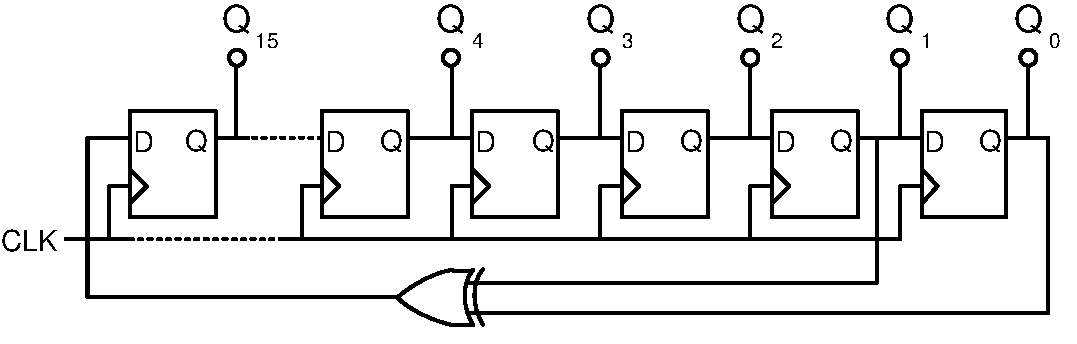
\includegraphics[width = 0.8\textwidth]{LFSR.pdf}
   \caption{16 Bit Linear Feedback Shift Register.\todo[inline]{Maybe change to IEEE symbols if we have time}}
   \label{fig:circles}
\end{figure}

An 2 input XOR gate is simulated by using masking the register value the comparing against inputs $00$ and $11$.\todo{surely this we can just use the XOR instruction}
These would return zero so only a shift is performed.
If this is not true then a shift is performed followed by an OR operation with $0$x$8000$ therefore feeding back a value to the top of the shift register.
This is described using C in listing~\ref{lst:random.c}. 

\lstinputlisting[style=C,label=lst:random.c,caption=Linear Feedback Shift Register Subroutine]{pseudocode/random.c}





\subsection{Interrupt}
The code for the interrupt program is held in Appendix~\ref{sec:interrupt_appendix} listing~\ref{lst:interrupt.asm}.
This is the most complex example and makes use of both the multiply and factorial subroutines in sections~\ref{sec:multiply} and~\ref{sec:factorial} respectively.

\lstinputlisting[style=C,label=lst:interrupt.c,caption=Serial Device Interrupt Service Request]{pseudocode/interrupt.c}




